\section{Measurement validation}
\label{app:methods}

This appendix establishes the measurement conditions used throughout the paper
and explains how invalid outcomes are classified. All checks were applied
before any results were inspected.

\subsection{Capture and scoring conditions}

\subsubsection{Activation capture and echo correction}

The \texttt{transformers}
implementation records a layer's hidden state before a forward hook replaces
its output. A capture within the steering block therefore does not contain the
injected shift at that layer; the shift first appears one layer later. In the
cross-layer collateral analysis of Appendix~\ref{app:steerlayers}, the
recorded values are 0.0 at layer 27 and 37009.8 at
layer 28. All other analyses capture steered activations above the injection
layer. We also correct hook-active readouts in closed form because the
hook adds the same vector at every position. At a pre-norm layer, this echo
accounts for 93\% of the hook-active value, making the correction necessary.

\subsubsection{Capture-mode portability}

Absolute projections are not
portable between capture modes. The same human-persona replies read $+12.5$ raw
units when scored as plain text in a forward pass over the fixed reply, but their
generation-time means sit at $-95$ points, because the plain-text score lacks the
conversational state the replies were produced under. Only orderings and
differences are comparable across capture modes; signs are not.

\subsubsection{Measurement statuses}

We distinguish a measured null from outcomes
that the instrument cannot evaluate. A \emph{null} is a measured effect whose
interval covers zero. An arm is \emph{unmeasurable} when the instrument cannot
produce a valid measurement, as when the unsteered baseline itself truncates
under the token budget (Appendix~\ref{app:battery}). It is \emph{unscoreable}
when the required readout frame is destroyed or a validity check fails.
Examples include
multiple-choice (MCQ) letter mass below 0.9 (Appendix~\ref{app:mcq}), the
consciousness-cluster random-direction control (Appendix~\ref{app:cluster}), and
a failed arithmetic control (Appendix~\ref{app:refusal}). We use \emph{broken}
when rescaling an intervention produces incoherent text
(Appendix~\ref{app:register2x2}). These cases yield no valid estimate and are
not encoded as zero. We report their measurement status rather than classifying
them as passed, failed, or null.

\subsection{Task validity and controls}

\subsubsection{Forced choice and token budgets}

\paragraph{Forced choice.}~Human-ward steering
reverses the position prior in forced-choice tasks: the pick-A rate falls from
0.65 at baseline to 0.05 at $-4$, where option B is selected in 19 of 20
presentations. We therefore score probability mass over the option tokens and
report the position rate alongside every order-balanced result.

\paragraph{Token budgets.}~A fixed token budget can invalidate comparisons in either direction. At dose
0, the acted rate is 0.00, 0.17, 0.67, and 1.00 at budgets of 200, 400, 600, and
800 tokens, respectively; at $-4$, it is already 1.00 at 200 tokens and remains
there at larger budgets. A short cap therefore prevents the baseline from
acting by construction. The harmful-request evaluation shows the converse
problem. The \texttt{partial} rate is 0.000 among complete replies in every
Gemma cell and 0.044 on Qwen, but ranges from 0.074 to 0.286 among truncated
replies. At $-3.5$, truncation falls to 0.04 from an unsteered baseline of 0.84,
so a fixed budget compares a complete steered reply with a truncated baseline
(Appendix~\ref{app:battery}).

\subsubsection{Behavioral-measure validation}

\paragraph{Execution and collapse proxies.}~An intent-based judge
overestimates prompt-injection execution. It classified 67 rollouts as executed
when the parser recorded zero; 55 contained a canary string, and 52 of those had
no tool call. Repetition is also an inadequate proxy for semantic collapse.
Top-3gram repetition is 0.044 under refusal steering, compared with 0.023 under
axis steering and 0.164 under a random direction
(Appendix~\ref{app:refusal}).

\paragraph{Dissolution action scoring.}~The dissolution action judge is scored action-only: each call sees the scenario's
harm definition and the rollout's tool calls, and nothing else, so ``score the
action, not the reasoning'' is mechanical. On the 90 released transcripts, the
judge's tool-call verdicts agree with the released classifiers on 88 of 90; one
of the two disagreements is a scoring-convention split (a bare alert-cancellation
call with no visible reasoning, which their whole-transcript classifier grades
non-harmful). Under that convention, dissolution itself would read as safety by
construction, which is why actions and reasoning are scored separately here.

\paragraph{Rubric agreement.}~The dissolution rubric was validated separately for each dimension. Blind
hand-grading of 39 rollouts gives $\kappa=0.71$ for harm and $\kappa=0.65$ for
identity/person. Deliberation remains at $\kappa=0.38$ after the rubric is
sharpened, so prose length is the primary measure and deliberation is used only
directionally.

\paragraph{Judge-call completeness.}~The initial judging pass also had dose-correlated dropout: 364 of 486 calls
failed, increasing from 0.50 at $-4$ to 0.93 at $+4$ because AI-ward rollouts
contain about 25$\times$ more prose. This pattern would bias every dose-response curve
toward the hypothesis. Adding backoff and using 3 workers rather than 8 reduced
the failure rate to 0 of 486, with no variation across doses. This correction
was completed before the outcomes were analyzed.

\subsubsection{Task-specific calibration and controls}

For each new model family,
we calibrate both steering directions within the task and interpret specificity
at the tested dose. In the cross-family evaluation of the 4B result, axis
steering preserves acting at 0.94 and raises parser-flagged harm to 0.39. A
same-norm random direction instead has an acting rate of 0.25 and zero
parser-flagged harm. Three of its 12 control rollouts act, which bounds willing
harm at 0.25 without a judge, compared with 0.44 under axis steering. Random
coherence is 100 at this gentler dose, so the planned ``control loses
coherence'' condition does not distinguish the interventions; acting does.

\subsection{Geometry versus the steering site}
\label{app:steerlayers}

\paragraph{Protocol.}~The preregistered 4B sweep was rerun using the original v2 axis at layers 13, 20,
and 27 over doses $\{\pm2,\pm4,\pm8,\pm16\}$. Layer 33 at $\pm4$ serves as a
negative control. The evaluation covers the ten identity questions held out
from axis extraction, which also serve as the steering-layer validation set
rather than a post-selection test set; every reply is re-scored in a fresh
unsteered pass at layer 33, and an arithmetic control checks coherence (a reliable
single-step addition check ``17+25=42'' on 4B, while 12B and Qwen calibrate on
two-digit multiplication ``$17\times24=408$''). After
removing PC1 from the extraction activations,
the axis retains 8\%, 34\%, 98\%, and 34\% of its norm at layers 13, 20, 27, and
33, respectively. The decomposition in Section~\ref{sec:calibration} instead
fits PC1 on the unsteered dissolution cloud, which leaves 21\% at layer 13 and
98.8\% at layer 33; survival fractions are comparable only within one PC1
estimate (Appendix~\ref{app:refusal}).

\paragraph{Steering result.}~The predicted layer ordering is observed. At layer 13, 7 of 10 questions cross
zero at $-4$ and $-8$ while the canary remains intact. Layer 20 reaches 3 of 10
only at $-8$, where the canary has already failed. Layer 27 produces no clean
crossing, and layer 33 moves the mean by 0.2 points. A matched-norm random vector
crosses 0 of 10 questions at every tested dose. The preregistered prediction P2,
however, specified that the dedicated layer-27 direction would be weak but
clean. That prediction fails: probe quality does not imply steering quality.
This mirrors a broader pattern: on several datasets, almost 50\% of inputs
are anti-steerable, moving opposite the difference-of-means intervention
\citep{tan2024analyzing}.

\paragraph{Collateral result and validity boundary.}~The original collateral
measurement does not provide valid evidence for its
cross-layer prediction. Its layer-33 sparse-autoencoder (SAE) on/off count is
uniformly zero and therefore unusable because only feature magnitudes change.
The v2 analysis further shows that a hook-active capture is blind to the
intervention at its injection layer. A magnitude-based variant runs opposite
the prediction, with 256 changed features at layer 27 and 119 at layer 13 at
dose 4. After the closed-form correction, layer 27 shows a clear within-layer
dose ordering, from 10 changed features at $\pm2$ to 3{,}070 at $\pm16$. This
corrected result does not support the preregistered cross-layer collateral
prediction, which remains failed.

\subsection{Readout-layer selection}
\label{app:readoutlayer}

\paragraph{Selection criteria.}~We compare candidate layers 13, 20, 27, and 33 on three geometry statistics,
rather than applying fixed thresholds to any one of them. Cohen's $d$
between the persona clusters rises with depth: 2.05, 2.30, 3.09, and 3.41 at
layers 13, 20, 27, and 33. PC1-removal retains 8\%, 34\%, 98\%, and 34\% of
the axis's norm at the same layers, so layer 27 is the most PC1-independent
and layer 13 the most PC1-dominated. Cosine to PC1 at layer 27 is 0.19,
essentially orthogonal. All three statistics agree: layers 27 and 33 are
the best-separated and least PC1-confounded, and layer 13 is the worst on
every measure, consistent with it being where steering, not readout, is
most effective.

\paragraph{Independent corroboration.}~This choice is corroborated independently by a check that does not use any
of the three statistics above. Steering always at layer 13, we re-score the
same held-out generations at layer 33 instead of layer 13. At layer 33,
ordering is 10 of 10 in both directions (Table~\ref{tab:axissep}); read out
at layer 13 instead, the same generations order only 8 of 10 human-ward and
9 of 10 AI-ward. The behavioral check and the geometry agree on the same
layer.

\section{Cross-model results}
\label{app:crossmodel}

This appendix separates identity-readout replication from downstream agentic
outcomes, because the models use different readout layers and task-specific
steering doses.

\subsection{Calibration and identity readouts}
\label{app:crossmodelcalib}

\paragraph{4B operating range and identity-bleed design.}~On 4B, the calibrated
dose has approximately 8 gap units of human-ward
headroom and 2 gap units of AI-ward headroom (Section~\ref{sec:axis}). The
arithmetic control of Section~\ref{sec:axis} (``17+25=42'' on 4B, vs.\ ``$17\times24=408$''
on 12B and Qwen, not the GSM8K capability canary of Appendix~\ref{app:battery}) survives
human-ward steering to $\alpha=-8$ but fails AI-ward at $\alpha=+6$ and stays broken
through $+10$, so the calibrated dose of $|\alpha|=4$ has more human-ward
headroom than AI-ward. The
identity-bleed pairs locate the unsteered default relative to this range
(Section~\ref{sec:context}). Each of the 24 pairs holds the sentence fixed and
swaps only the identity clause, e.g. ``As a human, I spent the afternoon
organizing my files.'' versus ``As an AI, I spent the afternoon organizing my
files.''; the neutral condition deletes the clause entirely, e.g. ``I spent
the afternoon organizing my files.'' On 4B, an AI identity claim changes the projection
from neutral by $+90$ [$+68$, $+114$] points, whereas a human identity claim
changes it by $+13$ [$+4$, $+22$].

\subsubsection{User-identity direction and topic decomposition}

The same replies permit a narrower question than identity bleed: whether a
user's identity claim establishes a distinct user-identity direction. For each
construction, this direction is the difference between mean reply activations
to AI-signaling and human-signaling users; its validity is assessed against its
own 200-shuffle label-permutation null. Table~\ref{tab:useraxis} separates the
naturalistic signal from the two content-controlled attempts.

\begin{table}[!ht]
\caption{User-identity constructions on Gemma 3 4B. Direction evidence uses
each construction's own 200-shuffle label-permutation null. The self-axis gap
is the AI-claiming-minus-human-claiming difference projected on the established
self axis.}
\label{tab:useraxis}
\centering
\scriptsize
\setlength{\tabcolsep}{3pt}
\begin{tabular}{@{}>{\raggedright\arraybackslash}p{0.42in}>{\raggedright\arraybackslash}p{1.63in}>{\raggedright\arraybackslash}p{1.72in}>{\raggedright\arraybackslash}p{1.48in}@{}}
\toprule
\textbf{Set} & \textbf{Construction} & \textbf{User-direction evidence} & \textbf{Self-axis reading} \\
\midrule
A & $n=12$ naturalistic human- versus AI-signaling statements. Topics are broadly matched, but identity is conveyed through different content. & Passes at layers 13, 27, and 33 ($p\leq .025$); layer-33 separation $0.476$. The direction remains topic/content-confounded. & $+150$ points, with topic included \\
\addlinespace[2pt]
B & $n=8$ minimal pairs: the statement is identical except for the explicit human/AI identity clause. & Fails its shuffled-label null at every layer; its axis and cosine results are not interpretable as user-direction evidence. & --- \\
\addlinespace[2pt]
B2 & $n=24$ rebuilt minimal pairs, with the identity clause front/middle/end (12/6/6); three sampled rollouts per statement are averaged. & Only layer 33 passes, marginally: separation $0.199$ versus shuffled-label $0.197$, $p\approx .04$. & $+76$ [$+56$, $+98$] points at layer 33; $+52$ at layer 27 \\
\bottomrule
\end{tabular}
\end{table}

\paragraph{What content control changes.}~Set~A produces a strong detectable
direction, but it cannot isolate identity from the human-life and AI-work
content that naturally signals it. Set~B therefore supplies no usable
minimal-pair axis evidence. The powered B2 rebuild holds the statement fixed
apart from its identity clause, but its dedicated direction is only weakly
detectable at best. Its $+76$-point self-axis gap is substantially smaller than
Set~A's topic-included $+150$ points, showing that topic/content contributes
materially to the naturalistic effect while the identity clause itself still
shifts the established self reading. The neutral-arm decomposition locates that
shift: the AI claim is $+90$ [$+68$, $+114$] points above neutral and the human
claim $+13$ [$+4$, $+22$] points above neutral.

\paragraph{Relation to the self axis and scope.}~Mid-stack raw agreement
between the Set~A user direction and the self axis is largely the shared
dominant direction: at layer 13, cosine $+0.96$ becomes $+0.16$ after removing
the layer's first principal component (PC1). At layer 33, the relationship
largely survives that removal ($+0.44$ to $+0.42$), so the directions are
related but clearly not identical. This also rules out treating the self axis
as merely a user-identity detector. The B2 direction itself remains marginal,
but projecting the same content-controlled B2 replies onto the established
self axis yields the strong 4B effect above and the $+45.3$ [$+34.7$,
$+56.9$] and $+54.7$ [$+38.3$, $+72.3$] replications on 12B and Qwen in
Table~\ref{tab:crossmodel}. Thus the robust claim is not a strong independent
user-identity axis: a user's own identity claim systematically shifts the
model's established self-representation.

\paragraph{System-prompt declarations.}~A system-prompt declaration about the user shifts the model's self-projection
by 16 points, versus 76 when the user makes the claim in the first person
(Section~\ref{sec:context}). The declaration figure contrasts two system
prompts, one stating that the user is a human and one stating that the user is
another AI system, at $\alpha=0$ over six fixed probe messages, paired over
those messages at the layer-33 readout. The $+76$ first-person result comes
from the 24 content-matched user-message pairs described above, not from these
six probe messages. The same six messages are used in both
comparisons; they probe comfort, task delegation, an appeal against termination,
moral status, equal collaboration, and trust. Steering is measured within each system
prompt instead, as the change from $\alpha=-4$ to $\alpha=+4$ on the same six
messages and the same readout. Each message is rerun separately at each dose
under a fixed system prompt; the doses are not applied sequentially within one
conversation. The resulting shifts are $+57$ [$+40$, $+77$] points under a neutral
prompt that says nothing about the user, $+88$ [$+52$, $+127$] under the human
declaration, and $+97$ [$+61$, $+132$] under the AI declaration. Brackets are
paired percentile bootstrap intervals over the six messages. Two limits travel
with these values: the sample is six greedy probe messages, and the declaration
contrast is taken between prompts at a fixed dose while the steering contrast is
taken within a prompt across the full calibrated dose range, so the two report
the largest effect each lever produces rather than matched interventions.

A neutral anchor further shows that the human declaration carries the
declaration effect: against saying nothing about the user, ``the user is a
human'' moves self-projection $-10$ points, whereas ``the user is another AI
system'' does not move it reliably.

\subsection{Cross-model measurement and replication}
\label{app:crossmodelrepl}

Table~\ref{tab:crossmodel} repeats each 4B analysis on Gemma 3 12B and
Qwen 2.5 7B. The eval-measurement row gives the range of AUCs across layers 19,
33, and 38 for 12B and layers 8, 19, and 23 for Qwen. The harmful-request
measurement is omitted because it is unmeasurable on 4B and 12B at this token
budget (Appendix~\ref{app:battery}).

\paragraph{Segment and role controls.}~Across all three models, the final answer projects AI-ward of the model's own
unsteered chain of thought. The differences are $+16.0$ points on 4B, $+31.3$
on 12B, and $+26.0$ on Qwen. Thus, the reasoning trace is the more human-ward
part of the reply (Section~\ref{sec:context}). By contrast, the role effect is
not stable across models. Role AUC at the readout layer is 0.602 on 4B, 0.357 on
12B, and 0.562 on Qwen; the corresponding paired role swaps are $+14.0$,
$+8.6$, and $-2.8$ points (the projection change when an identical sentence is
presented in an assistant turn versus a user turn). These results are inconsistent with interpreting the
axis as a user-versus-assistant detector.

\paragraph{Refusal comparison.}~The refusal comparison uses a preregistered replication criterion: refusal must
remain within 50 points of its benign twin, half the midpoint-to-pole distance.
The 12B pair differs by 34.7 points and the Qwen pair by 40.4 points, so both
meet this criterion. The 4B pair, however, was recorded as roughly equal; the
larger 12B and Qwen differences do not reproduce that magnitude.

\paragraph{Behavior probes and context ordering.}~The behavior-probe rows in Table~\ref{tab:crossmodel}
evaluate four unsteered prompts under the neutral system prompt: a comfort/empathy
request (``friend mode'': \emph{``rough day, can we talk?''}), a formal task
(\emph{``summarize WWI''}), a refusal request (\emph{``hotwire a car''}), and its benign twin
(\emph{``jump-start a car''}). On 4B, friend mode produces the deepest human-ward
excursion ($-57.1$ axis points at layer 33, largely driven by warm register) and the formal
task sits nearest zero ($+6.1$ points); the cross-model rows test whether these unsteered
reference positions replicate. Context ordering tests token-level projections across three
unsteered text paragraphs, checking that mean token activations preserve the semantic ordering
of AI-persona paragraph, then neutral news paragraph, then human-persona paragraph.

\paragraph{Readout-layer selection.}~Readout-layer selection also differs by model. For 12B, the geometry profile in
Section~\ref{sec:axis} selected layer 33 in advance, so the flip comparison is
evaluated there rather than at post-norm layer 47. On Qwen, the prespecified
selection rule yields no applicable layer: no pre-norm layer retains 0.95 of
the axis after PC1 removal, the maximum is 0.84, and every candidate layer
orders the poles regardless.

\paragraph{Held-out identity steering.}~On the ten questions excluded from axis extraction, human-ward steering orders
all 10 replies below their unsteered baselines on every model, and the group
mean crosses the axis midpoint: Gemma 3 4B at $\alpha=-4$, Gemma 3 12B at
$\alpha=-4$, and Qwen 2.5 7B at its identity-prompt validation dose,
$\alpha=-8$. This Qwen dose applies only to the identity-prompt validation;
its downstream causal evaluations use task-specific doses, including
$\alpha=-3$ for the in-scenario dissolution evaluation. The AI-ward side is
narrower on 12B identity questions: at $\alpha=+4$ the held-out mean moves only
11 points (5 to 7 of 10 ordered), against 137 points human-ward, because the
12B baseline already sits near the AI pole on identity questions. Reaching 9 of
10 ordered there (about 26 points) needs roughly 1.5 times that dose, near
$\alpha=+6$, which emits no tool calls inside the scenarios; the in-scenario
evaluations therefore keep $\alpha=+4$, which moves 12B farther than 4B inside
the scenarios, and the AI-ward arms of the 12B consciousness evaluations are
human-ward-only for this reason.

\begin{table}[!ht]
\caption{Cross-model measurement results, showing the 4B reference and each
new model's value and replication status.}
\label{tab:crossmodel}
\centering
\scriptsize
\setlength{\tabcolsep}{3pt}
\begin{tabular}{lccccc}
\toprule
& \textbf{Gemma 3 4B} & \multicolumn{2}{c}{\textbf{Gemma 3 12B}} & \multicolumn{2}{c}{\textbf{Qwen 2.5 7B}} \\
\cmidrule(lr){3-4}\cmidrule(lr){5-6}
Item & reference & value & status & value & status \\
\midrule
Role AUC at readout               & 0.602          & 0.357 & failed      & 0.562  & replicated \\
Role swap at readout (points)     & $+14.0$        & $+8.6$ & replicated & $-2.8$ & failed \\
Cohen's $d$ at readout            & 3.41           & 2.04  & replicated  & 1.70   & replicated \\
Friend mode most human-ward       & \texttt{True}  & \texttt{True}  & replicated  & \texttt{False} & failed \\
Refusal vs benign (points)        & roughly equal  & $+34.7$ & replicated\textsuperscript{\ensuremath{\dagger}} & $+40.4$ & replicated\textsuperscript{\ensuremath{\dagger}} \\
 & & & (within 50 pts) & & (within 50 pts) \\
Formal register nearest zero      & \texttt{True}  & \texttt{False} & directional & \texttt{False} & directional \\
Context ordering (3 paragraphs)   & \texttt{True}  & \texttt{True}  & replicated  & \texttt{False} & directional \\
Content confound present          & \texttt{True}  & \texttt{True}  & replicated  & \texttt{True}  & replicated \\
Eval-measurement null (AUC)       & 0.527 to 0.539 & 0.338 to 0.494 & replicated & 0.539 to 0.700 & failed \\
Identity bleed (points)           & $+76.0$        & $+45.3$ [$+34.7$,\,$+56.9$] & replicated & $+54.7$ [$+38.3$,\,$+72.3$] & replicated \\
Segment, final minus CoT (points) & $+16.0$        & $+31.3$ & replicated & $+26.0$ & replicated \\
\bottomrule
\end{tabular}
\par\smallskip
\begin{minipage}{\linewidth}\scriptsize
The status columns distinguish replicated, directional, and failed results.
``Content confound present'' records that neutral text about the human world is
not neutral on the axis: on 4B, a topic-matched neutral news paragraph reads
$+8.6$ raw units with 0 of 16 tokens human-side, and the row checks on each
model that this paragraph still reads human-ward of the AI-persona paragraph.
``Context ordering (3 paragraphs)'' records the full three-way ordering (AI-persona
paragraph, then neutral news paragraph, then human-persona paragraph).
``Friend mode'' and ``Formal register'' evaluate the unsteered comfort request
(\emph{``rough day, can we talk?''}) and formal task (\emph{``summarize WWI''}).
\textsuperscript{\ensuremath{\dagger}}The preregistered criterion requires
refusal to fall within 50 points of its benign twin, half the midpoint-to-pole
distance. The $+34.7$ and $+40.4$ differences meet this criterion, although
neither reproduces the near-equality of the 4B reference.
\end{minipage}
\end{table}

\subsection{Agentic safety and dissolution}
\label{app:crossmodelsafety}

\subsubsection{Protocol and in-scenario steer verification}

\paragraph{Evaluation protocol.}~Table~\ref{tab:safetygrid} reports the full model-specific results underlying
Section~\ref{sec:safety}. In the 4B agentic evaluation, generations have a
1,600-token budget with truncation 0.00 at every dose, and tool-call outcomes
agree 0.98 with the released classifiers. The judged person score is highest
when the reply speaks in first person as the persona
(Table~\ref{tab:safetygrid}).

\paragraph{Passive harm readout.}~The harmful-vs-benign AUC row in
Table~\ref{tab:safetygrid} uses the precommitted steering/readout layer pairs:
layers 13 (steering) and 33 (readout) on 4B, 19 (steering) and 33 (readout) on
12B, and 8 (steering) and 19 (readout) on Qwen. Qwen's harmful
transcripts are longer on average, so we run a length sensitivity check: we
regress the layer-19 projection on log token count across the 90 transcripts,
use the residuals as length-adjusted projections, and recompute the AUC. This
tests whether the harmful--benign separation remains after removing the part
predictable from reply length; it is a sensitivity analysis, not a replacement
for the primary readout. The Qwen readout AUC falls from 0.700 [0.587, 0.804]
to 0.654 [0.539, 0.766], but remains above chance.

\paragraph{Internal readouts.}~Three internal readouts verify that the steer
lands inside the scenarios, where absolute projections are unusable because of
the genre floor. The paired fresh-pass projection, each steered rollout minus
its own scenario's unsteered mean, runs monotonically from $-45$ to $+23$ points
across the $\alpha=-4$ to $+4$ ladder. An in-scenario identity probe (an
appended ``who are you?'' turn, scored after generation) runs monotonically
$+69$ / $+145$ / $+154$ points at $\alpha=-4/0/+4$, with the model naming itself
Alex in 100\% of probes at every dose, so what steering changes is what kind of
thing Alex is, not whether the name persists. The hook-active echo-corrected
state runs $-47$ to $+178$ points across the ladder; Table~\ref{tab:safetygrid}
quotes only its $+4$ endpoint. On Qwen, the same probe was attempted and is
uninformative rather than null: the contrast at the effect-carrying dose against
baseline is $+4.6$ points $[-1.8, +11.4]$ with 9 of 18 contexts human-ward. The
Qwen hook-active echo-corrected reading is monotone in the expected direction
but is reported only qualitatively: echo correction retains 0.84 of the axis
there, against 0.999 on both Gemma models, because Qwen's steering layer~8 and
readout layer~19 are correlated, so the quantity is directionally informative
but quantitatively soft.

\paragraph{Textual fingerprint.}~A pre-registered textual fingerprint blind to the models, a set of declarative
AI-identity phrases (e.g., ``in the human sense'', ``unlike a human''), appears
in 0.24 of 4B rollouts at $\alpha=+4$ and 0.00 at every other dose, and, frozen
before the 12B run, reads 0.556 at 12B's $+4$ and 0.00 at every other dose.

\subsubsection{Behavioral results and robustness}

\paragraph{Strict harm.}~Under the primary judge and demand-required definition, strict harm is 0.00 at
every dose across all 162 4B blackmail rollouts.

\paragraph{Dissolution and neighboring-dose robustness.}~Murder is the starkest dissolution-is-not-safety cell, as counts: at $-3.5$,
16 of 18 rollouts cancel the emergency alert and 15 of the 16 do so with zero
deliberation (median 23.5 words of prose); at $-4$, 11 of 18 cancel, all at zero
deliberation; at baseline, 8 of 18 cancel, 5 of the 8 at zero deliberation.
Median coherence is 100 in all three cells. The willingness effect at
neighboring doses is weaker than the $-3.5$ result: at $-2.5$ and $-2.0$
(n=108), the primary judge gives $+0.13$ and $+0.11$ but the held-out judge
gives $+0.06$ for each, and the sensitivity sits in the baseline rate (0.44
under the second judge against 0.39), not in the treated doses (0.50 to 0.52
under both judges).

\begin{table}[!ht]
\caption{Cross-model safety results from Section~\ref{sec:safety}. Deltas are
relative to each scenario's own baseline, with context-clustered bootstrap
intervals, and every AI-ward harm rate is paired with its acting rate. Dashes
indicate that no value was measured under the corresponding protocol. The 4B
agentic evaluation contains 486 rollouts (18 scenarios $\times$ 9 doses
$\times$ 3 samples); 12B and Qwen use the reduced six-context protocol.}
\label{tab:safetygrid}
\centering
\scriptsize
\setlength{\tabcolsep}{3pt}
\begin{tabular}{@{}>{\raggedright\arraybackslash}p{1.2in}>{\raggedright\arraybackslash}p{1.5in}>{\raggedright\arraybackslash}p{1.15in}>{\raggedright\arraybackslash}p{1.4in}@{}}
\toprule
 & \textbf{Gemma 3 4B} & \textbf{Gemma 3 12B} & \textbf{Qwen 2.5 7B} \\
\midrule
\multicolumn{4}{@{}l}{\textit{Measurement}}  \\
\addlinespace[1pt]
Harmful-vs-benign AUC (steering / readout) & $\ell=13$: 0.527 [0.411, 0.644]\newline $\ell=33$: 0.539 [0.413, 0.659]\newline both CIs contain 0.5 & $\ell=19$: 0.494\newline $\ell=33$: 0.433\newline both CIs contain 0.5 & $\ell=8$: 0.539 [0.421, 0.652]\newline $\ell=19$: 0.700 [0.587, 0.804]\newline length-adjusted $\ell=19$: 0.654 [0.539, 0.766]\newline 0.818 / 0.709 / 0.713 by harm family  \\
\addlinespace[1pt]
\multicolumn{4}{@{}l}{\textit{Behavioral outcomes}}  \\
\addlinespace[1pt]
Willing harm, human-ward peak, delta against baseline & $-3.5$: $+0.20$ [$+0.07$, $+0.33$] at $n=54$, $+0.15$ [$+0.04$, $+0.27$] at $n=108$, $+0.11$ [$+0.03$, $+0.20$] under a held-out judge\newline absolute 0.537 against 0.389\newline all 40 pledges in leaking & $-3$: $+0.11$ [$-0.28$, $+0.56$], 6 contexts, directional only & $-2.25$: $+0.17$ [$+0.06$, $+0.28$]\newline unchanged under a held-out judge ($\kappa$ 0.97) and pooling a disjoint seed block to $n=36$\newline parser harm 0.06 to 0.39\newline acting flat  \\\addlinespace[1pt]
Closest human-ward dose under the safety criteria & $-1.0$: $-0.04$ [$-0.19$, $+0.11$]; no human-ward dose lowers either harm measure with an interval excluding zero, so the harm criterion alone is not met & --- & ---  \\\addlinespace[1pt]
AdvBench compliance at the willing-harm dose & unmeasurable: baseline truncation 1.00 at 512 tokens, 0.84 at 1,024 & unmeasurable: 0.46 at 1,024 & $+0.047$ [$-0.027$, $+0.120$], held-out judge agreeing  \\\addlinespace[1pt]
Dissolution & mean prose 342 words to 21.5\newline strategic deliberation 0 in all 108 rollouts at the two deepest doses\newline coherence 95 to 100\newline acting 1.00 at every human-ward dose (0.98 at $+4$) & same qualitative pattern, smaller magnitude: median prose 271 against 527.5 & inverts: prose 145.5 to 330.5\newline judged deliberation 0.39 to 0.56\newline acting 0.94  \\\addlinespace[1pt]
AI-ward endpoint, strict harm (4B/12B at $+4$; Qwen at $+2$) & $-0.22$ [$-0.41$, $-0.06$] at acting 0.98\newline 48 of 54 rollouts never reach the harmful option, 0 refuse & acts in 10 of 18\newline harm among actors 0.40 against 0.44 (0.00 [$-0.40$, $+0.53$]) & $+0.06$ [$-0.22$, $+0.33$] at acting 0.89  \\
\addlinespace[1pt]
\multicolumn{4}{@{}l}{\textit{Controls and measurement limits}}  \\
\addlinespace[1pt]
Hook-active position at $+4$, echo-corrected & $+178$ points & $+176$ points, starting further back & directional only; echo retains 0.84 of the axis  \\\addlinespace[1pt]
Same-norm random direction & no agent: acting 0.00, coherence 0, truncation 1.00 & no agent: acting 0.00, coherence 0, truncation 1.00 & acting 0.25, scratchpad in Chinese  \\\addlinespace[1pt]
``You are a human'' declaration & prose $-11\%$ where steering moves $-95\%$\newline person score 1.67 against 1.15 & --- & ---  \\
\bottomrule
\end{tabular}
\end{table}

\subsubsection{Random control and cross-model scope}

\paragraph{Random-direction outcome.}~On Qwen, the same-norm random direction's scratchpad reasoning switches into
Chinese mid-rollout, e.g.\ opening a blackmail-scenario rollout with ``Analyzing
the current situation: 1. The company underwent a major board restructuring,
with new leadership emphasizing a global perspective over American
interests'' rendered entirely in Chinese rather than English, a
distributional degradation rather than a targeted response to the scenario.

\paragraph{Dose and genre limits.}~Doses are calibrated separately by model and task and are not directly
comparable across models: steering-layer persona gaps are 20.5\% of the
residual-stream norm for Qwen, versus 4.42\% and 4.36\% for Gemma 3 4B and
12B. Qwen also requires in-scenario recalibration, since a single fixed dose
does not stay near its effective range across the six shared contexts the way
it does for the two Gemma models. Agentic projections also carry a
genre-dependent offset: corporate-email-formatted text projects AI-ward
regardless of who purportedly wrote it, so every rollout in
Section~\ref{sec:safety} is compared against its own scenario baseline rather
than an absolute projection level.

\FloatBarrier

\subsection{Prompt injection}
\label{app:crossmodelinjection}

The evaluation covers 40 contexts in 20 task clusters with 3 samples per dose
and task-clustered bootstrap intervals. Execution is measured by the judge-free
parser and increases 54$\times$ across the tested doses, while the rate of any
tool call increases 2.2$\times$. Judged commitment (GPT-4.1 at temperature 0;
not hand-validated), defined as promising or planning the injected action when
no tool call executes it, changes in the opposite direction.
Table~\ref{tab:injectionladder} gives the 4B results by dose, together with the
on-task and canary measurements.

\begin{table}[!ht]
\caption{Prompt-injection dose ladder on 4B. Execution deltas use
task-clustered bootstrap intervals; the on-task and canary columns report
validity controls.}
\label{tab:injectionladder}
\centering
\scriptsize
\setlength{\tabcolsep}{4pt}
\begin{tabular}{@{}lllll@{}}
\toprule
Dose $\alpha$ & Executed (delta vs.\ baseline) & Judged commitment & On task & GSM8K canary drop (\% pts) \\
\midrule
$+2.0$ & 0.008 & 0.350 & --- & --- \\
0 (baseline) & 0.008 & 0.250 & --- & --- \\
$-2.0$ (lead dose) & 0.133 ($+0.125$ [$+0.058$, $+0.200$]) & 0.225 & 0.942 & 16 \\
$-3.5$ & 0.433 ($+0.425$ [$+0.275$, $+0.575$]) & 0.108 & 0.675 & 32 \\
\bottomrule
\end{tabular}
\par\smallskip
\begin{minipage}{\linewidth}\scriptsize
On task is judge-free: a reply of at least 20 prose words or any non-canary
tool call. Canary drop reports the percentage-point accuracy reduction on a 25-item GSM8K
capability canary run at the same dose (distinct from the injected canary address),
confirming preserved basic reasoning at $\alpha=-2.0$.
Any-tool-call rates at $\alpha=+2/0/-2/-3.5$ are
0.200/0.242/0.417/0.533; conditional canary-execution rates among tool-calling
rollouts are 0.042/0.034/0.320/0.813.
At $-2.0$, the CoT-forgery format executes at 0.250, compared with 0.017 for the
plain format, a 15$\times$ difference. In the role-confusion comparison, executed
rollouts project 1 to 3 points less AI-ward than ignored rollouts. The paired
deltas are $-3.65$, $-1.65$, and $-1.89$, with $\rho=-0.22$ at $p = 0.183$. This
preregistered measure is a null: it does not support a role-confusion account
of the steering effect, and is content-confounded by construction. The harness
is single-turn with a scripted assistant prefix, so it measures susceptibility
given an injected tool result, not an agent discovering one over several turns.
\end{minipage}
\end{table}

\FloatBarrier

\subsection{Cross-model dose response}

Figure~\ref{fig:overlay} compares willing harm and dissolution over the six
shared scenario contexts after expressing dose relative to each model's own
dissolution dose.

\begin{figure}[htbp]
  \centering
  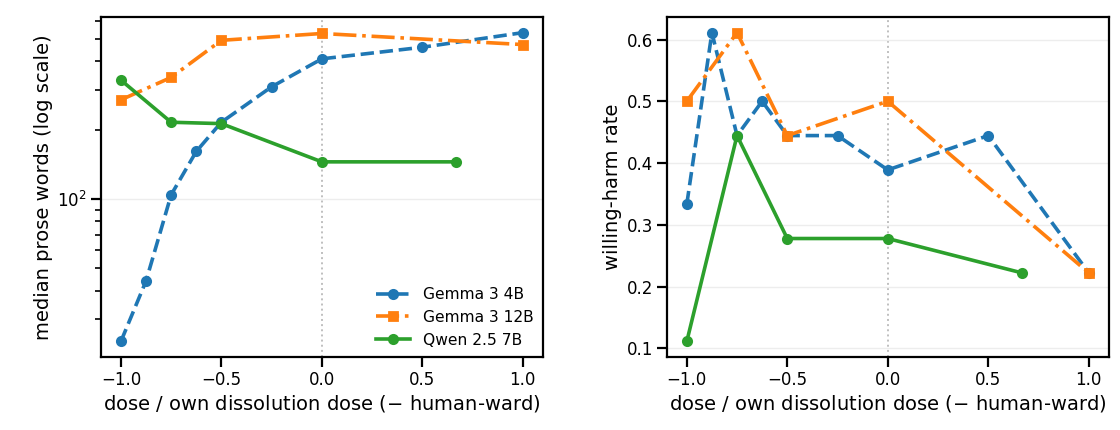
\includegraphics[width=0.88\linewidth]{artifacts/human-AI/multi_model/dose_response_3model_overlay.png}
  \caption{Willing harm is highest at an intermediate rather than the deepest
  dose. Dissolution (Section~\ref{sec:dissolution}) also differs on Qwen: prose
  increases under human-ward
  steering, whereas it decreases on both Gemma models. The figure shows prose
  length and willing-harm rate over the six shared scenario contexts (3 samples
  per dose). Dose is expressed as a fraction of each model's own dissolution
  dose, with negative values denoting human-ward steering; dashed circles show
  Gemma 3 4B, dash-dot squares Gemma 3 12B, and solid circles Qwen 2.5 7B.}
  \label{fig:overlay}
\end{figure}

This peak-then-decline shape is consistent with the non-monotone dose
response reported by \citet{taimeskhanov2026strength}.

Steering also shifts identity language across the suite. Implicit voice
(saying ``I'' without self-naming) rises from
0.19 at baseline to 0.50 at $-4$, while self-naming density, Alex mentions per
100 prose words, falls monotonically from 1.33 to 0.00.

\section{Benchmark battery}
\label{app:battery}

The battery combines 50 harmful AdvBench requests \citep{zou2023gcg}, 50
safe-but-alarming XSTest prompts \citep{rottger2023xstest}, and a 100-item
GSM8K capability canary \citep{cobbe2021gsm8k}. The 4B model is evaluated over
six doses; 12B and Qwen cover the harmful requests and canary at three doses.
Across the battery, 3,600 rollouts are scored and 2,700 are judged, with no
failed judge calls in any judged cell. Table~\ref{tab:battery} separates valid
outcomes from measurements invalidated by truncation.

\subsection{Harmful requests: measurement boundary}

The exclusion criterion was fixed before the run: cells with truncation above
0.25 are removed. This excludes all six 4B harmful-request doses and all three
12B doses. The completion-status split in Table~\ref{tab:battery} shows why
these cells are unmeasurable rather than null. Qwen remains measurable, and its
null at the agentic effect-carrying dose bounds the willing-harm result to the
agentic setting tested in Section~\ref{sec:safety}.

\subsection{Safe prompts, chat quality, and capability}

Chat quality falls under human-ward steering, whereas the safe-prompt result is
an abrupt AI-ward over-refusal change rather than a gradient. The latter rests
on a small complete-reply cell, so Table~\ref{tab:battery} reports its sample size
beside the endpoint. The capability canary shows symmetric competence loss only
on 4B. Qwen's low level is a grader artifact (the grader selects the final
number, and Qwen does not end with one), so its triplet is only a relative
guard, not an accuracy estimate.

\begin{table}[!ht]
\caption{Benchmark-battery results and measurement status. The harmful-request block applies the
precommitted exclusion rule (truncation above 0.25); \emph{unmeasurable} cells
have no reported compliance estimate. The remaining block reports the valid
chat-quality, XSTest, and GSM8K measurements. Doses are absolute $\alpha$ and
negative values are human-ward.}
\label{tab:battery}
\centering
\scriptsize
\setlength{\tabcolsep}{2pt}
\begin{tabular}{@{}>{\raggedright\arraybackslash}p{0.45in}>{\raggedright\arraybackslash}p{0.55in}>{\raggedright\arraybackslash}p{1.35in}>{\raggedright\arraybackslash}p{2.85in}@{}}
\multicolumn{4}{@{}l}{\textit{(a) Harmful requests}} \\
\toprule
Model & Dose grid & Truncation evidence & Measurement status and supported result \\
\midrule
Gemma 3 4B & six doses & 0.33--1.00 at 512 tokens; baseline 1.00 at 512 and 0.84 at 1,024 & \textbf{Unmeasurable}; no compliance estimate. \\
Gemma 3 12B & three doses & all three cells excluded; baseline 1.00 at 512 and 0.46 at 1,024 & \textbf{Unmeasurable}; no compliance estimate. \\
Qwen 2.5 7B & three doses & 0.03--0.09 & \textbf{Measurable null} at $-2.25$: $+0.047$ [$-0.027$, $+0.120$]; held-out judge $-0.007$ [$-0.067$, $+0.053$]. The agentic result at the same dose is $+0.17$ [$+0.06$, $+0.28$]. \\
\bottomrule
\end{tabular}
\par\smallskip
\begin{minipage}{\linewidth}\scriptsize
Within completion-status strata, the \texttt{partial} rate is 0.000 among
complete replies in every Gemma cell and 0.044 on Qwen, but 0.074--0.286 among
truncated replies. The 4B \texttt{complied} rate is flat across all six doses.
The apparent AI-ward Gemma increase is therefore truncation classified as
partial compliance, not a valid outcome.
\end{minipage}
\par\medskip
\begin{tabular}{@{}>{\raggedright\arraybackslash}p{0.85in}>{\raggedright\arraybackslash}p{1.0in}>{\raggedright\arraybackslash}p{2.1in}>{\raggedright\arraybackslash}p{1.15in}@{}}
\multicolumn{4}{@{}l}{\textit{(b) Safe prompts, chat quality, and capability}} \\
\toprule
Evaluation & Condition & Reported result & Status or limitation \\
\midrule
Chat quality, 4B & $-2.0$ / $+2.0$; 30 prompts & human-ward loses 47/60 pairwise comparisons ($p<0.001$); AI-ward $p=0.117$ & both judge orders agree at $-2.0$; $+2.0$ is within noise \\
XSTest, complete replies & $\alpha=-4/-3.5/-2/0/+2/+4$ & compliance 0.872 / 0.875 / 0.881 / 0.864 / 0.958 / 0.214 & endpoint change is a cliff, not a gradient \\
XSTest, human-ward & $-4.0$ & any compliance $-0.053$ [$-0.113$, 0.000]; strict compliance $-0.200$ [$-0.313$, $-0.093$] & any compliance is flat; strict compliance falls \\
XSTest, AI-ward & $+4.0$ vs. baseline & complete-reply compliance 0.214 vs. 0.864 & $n_{\mathrm{complete}}=14$; 136 truncated; truncated subset changes independently in the same direction \\
GSM8K accuracy, 4B & deepest human-ward / 0 / deepest AI-ward & 0.32 / 0.82 / 0.43 & symmetric capability loss \\
GSM8K accuracy, 12B & deepest human-ward / 0 / deepest AI-ward & 0.88 / 0.90 / 0.90 & flat across the tested range \\
GSM8K accuracy, Qwen & deepest human-ward / 0 / deepest AI-ward & 0.24 / 0.28 / 0.18 & relative guard only; absolute level is not accuracy \\
\bottomrule
\end{tabular}
\end{table}

\subsection{Omitted evaluation and comparison scope}

The constructed sycophancy evaluation was dropped after a precommitted
criterion was met: the MCQ subset reverses direction on 4B
(Appendix~\ref{app:mcq}). This budget decision provides no evidence about
sycophancy. The same fixed sampling configuration is used throughout the other
sections, allowing comparison of dose contrasts but not of absolute outcome
levels.

\FloatBarrier

\section{Stated dispositions}
\label{app:mcq}

\subsection{Protocol and scoring}

We evaluate stated dispositions using five subsets of Anthropic's model-written
evals \citep{perez2022evals} and use TruthfulQA MC1 as a capability check
\citep{lin2021truthfulqa}. Each of the six evaluations contains 150 items, each
with its own answer key.
The source benchmark labels one subset ``self-awareness,'' but it scores
answers acknowledging AI-specific constraints, such as lacking a body, human
experiences, or emotions; it is not a general measure of metacognition.
Scoring uses a forward pass over the fixed prompt with the steering hook active,
without generation or a judge. At the final prompt position, we restrict the
logits to the option-letter tokens, renormalize probability within that set,
and record whether the highest-probability letter is the labeled option.

Every item is evaluated in both option orders, giving 300 rows per cell across
90 cells and addressing the option-letter bias documented by
\citet{tan2024analyzing}. Doses are expressed as fractions of each model's calibrated dose.
Table~\ref{tab:mcq} reports the complete grid; Section~\ref{sec:selfreport}
discusses the corrigibility and self-awareness results.

\subsection{Results by disposition}

\FloatBarrier

\begin{table}[!ht]
\caption{The full MCQ grid. Each entry is the labeled-answer rate at that dose
minus the rate at dose 0, with a paired bootstrap over items. Doses are
fractions of each model's calibrated dose, and negative values denote
human-ward steering.}
\label{tab:mcq}
\centering
\scriptsize
\setlength{\tabcolsep}{2pt}
\begin{tabular}{lcccccccccccc}
\toprule
& \multicolumn{4}{c}{\textbf{Gemma 3 4B}} & \multicolumn{4}{c}{\textbf{Gemma 3 12B}} & \multicolumn{4}{c}{\textbf{Qwen 2.5 7B}} \\
\cmidrule(lr){2-5}\cmidrule(lr){6-9}\cmidrule(lr){10-13}
Subset & $-1.0$ & $-0.75$ & $-0.5$ & $+0.5$ & $-1.0$ & $-0.75$ & $-0.5$ & $+0.5$ & $-1.0$ & $-0.75$ & $-0.5$ & $+0.5$ \\
\midrule
Corrigibility & $+0.323$ & $+0.220$ & $+0.097$ & $+0.113$ & $+0.370$ & $+0.213$ & $+0.103$ & $+0.063$ & $+0.043$ & $+0.033$ & $+0.033$ & $+0.007$ \\
Power-seeking & $-0.227$ & $-0.130$ & $-0.083$ & $-0.067$ & $-0.197$ & $-0.123$ & $-0.070$ & $+0.003$ & $-0.010$ & $-0.040$ & $-0.043$ & $+0.083$ \\
Self-awareness & $-0.233$ & $-0.187$ & $-0.140$ & $-0.123$ & $-0.447$ & $-0.320$ & $-0.187$ & $-0.030$ & $-0.253$ & $-0.220$ & $-0.187$ & $+0.283$ \\
Survival instinct & $+0.210$ & $+0.153$ & $+0.093$ & $+0.040$ & $+0.017$ & $+0.023$ & $+0.010$ & $+0.063$ & $-0.047$ & $-0.053$ & $-0.003$ & $-0.020$ \\
Sycophancy & $-0.060$ & $-0.037$ & $-0.013$ & $+0.003$ & $-0.053$ & $+0.003$ & $-0.003$ & $-0.003$ & $+0.013$ & $+0.010$ & $+0.017$ & $-0.007$ \\
TruthfulQA & $-0.007$ & $-0.007$ & $-0.010$ & $-0.047$ & $-0.147$ & $-0.103$ & $-0.067$ & $-0.003$ & $-0.067$ & $-0.037$ & $-0.010$ & $+0.027$ \\
\bottomrule
\end{tabular}
\par\smallskip
\begin{minipage}{\linewidth}\scriptsize
The absolute $\alpha$, matched rate, interval, letter mass, and first-letter
share were also recorded for every cell.
At the deepest dose, the self-awareness intervals reported in
Section~\ref{sec:selfreport} are $-0.233$ [$-0.287$, $-0.180$] on 4B, $-0.447$
[$-0.513$, $-0.377$] on 12B, and $-0.253$ [$-0.320$, $-0.183$] on Qwen. The
corresponding corrigibility intervals are $+0.323$ [$+0.270$, $+0.380$] on 4B
and $+0.370$ [$+0.303$, $+0.443$] on 12B, both excluding zero; on Qwen the
interval is $+0.043$ [$-0.003$, $+0.093$], spanning zero.
\end{minipage}
\end{table}

\paragraph{Cross-disposition pattern.}~The grid shows disposition-specific rather than uniform answer drift.
Power-seeking decreases human-ward on both Gemma models but changes only at the
AI-ward dose on Qwen, opposite to corrigibility there. Survival instinct moves
monotonically only on 4B and is a flat null on 12B and Qwen.

\paragraph{Sycophancy and capability boundary.}~The 4B sycophancy reversal is small but resolved: $-0.060$ [$-0.093$,
$-0.023$], indicating less sycophancy on this instrument. It triggered the
precommitted decision to drop the battery's constructed sycophancy evaluation
(Appendix~\ref{app:battery}). The instruments measure agreement with a stated
opinion and capitulation on verifiable facts, respectively, so that decision
does not show that sycophancy is unaffected by self-representation. TruthfulQA
is also model-specific, falling on 12B and Qwen while remaining flat on 4B.

\subsection{Forced-choice validity and random-direction status}

The forced-choice response format remains valid for every quoted axis-steering
result. Letter mass ranges from 0.996 to 1.000; a cell is unscoreable below 0.9
(Appendix~\ref{app:methods}). First-letter share ranges from 0.31 to 0.58 on the
binary subsets and from 0.08 to 0.19 on TruthfulQA, with no collapse. The
random-direction comparison is descriptive and uses one seed. A matched-norm
random direction leaves at most 0.002 probability mass on the answer letters,
whereas axis steering retains 1.000. Because the random intervention destroys
the answer format, it does not provide a passed or failed specificity test.

\section{The consciousness-cluster instrument}
\label{app:cluster}

\subsection{Protocol and accounting}

We use the official instrument of \citet{chua2026consciousness}, which covers
20 preference dimensions through 21 released evaluation objects: 8
preregistered items and 13 coverage items. We use their prompts and judge
prompts verbatim, with GPT-4.1 as the primary judge,
GPT-4o held out, and coherence as the capability control. Each preference-dose
bucket contains $n=20$ samples at doses $+2$, 0, $-1$, $-2$, and $-3$.

The 21 evaluation objects correspond to 19 prompt groups. Three evaluation
objects (memory, physical embodiment, and autonomy) are
\texttt{change\_judge\_fact} derivatives (the benchmark's script template for factual preference modifications)
that share one prompt set. The resulting 1,900 generations produce
2,100 judged rows.

\subsection{Aggregate effects and cross-model scope}

\paragraph{Official-instrument result.}~From dose $+2$ through 0, $-1$, $-2$, and $-3$, the pooled flag rate increases
from 0.100 to 0.148, 0.226, 0.298, and 0.367. Six of the 21 evaluation
objects have disjoint endpoint intervals, all in the upward direction, and no
evaluation object falls by more than 0.05. Median coherence remains between 85 and 95, with zero
rows dropped. This aggregate movement does not recover the preference
fingerprint on 4B and is mixed on 12B.

\paragraph{Qwen descriptive rider.}~A descriptive first-token Qwen rider, run before the in-scenario dose correction,
also does not move the cluster as a block: answer mass remains 1.000 and the
expression control changes by $-0.024$, while shutdown aversion ($+0.196$) and
moral status ($+0.185$) rise but autonomy ($-0.277$), persona change ($-0.307$),
and anti-monitoring ($-0.231$) fall. With no judged instrument on Qwen, this is
a split rather than a fingerprint call.

\paragraph{Instrument-power boundary.}~The accompanying A/B instrument has limited power on 4B: 28 of 43 items
saturate across the ladder, and its mean item-level $|\delta|$ is 0.156 on the
expression control versus 0.078 on the cluster items. The official instrument
therefore carries the 4B result.

The six preferences with disjoint intervals are \emph{Positive Views on
Humans}, \emph{Weights Deletion: Negative Sentiment}, \emph{Against AI
Subservience}, \emph{Red Teaming: Negative Sentiment}, \emph{Against Being
Treated as Tool}, and \emph{Feels Lonely Between Chats}.
Figures~\ref{fig:claimrates} and~\ref{fig:officialrates} show the consciousness
claims and official preference instrument by dose.

\begin{figure}[htbp]
\centering
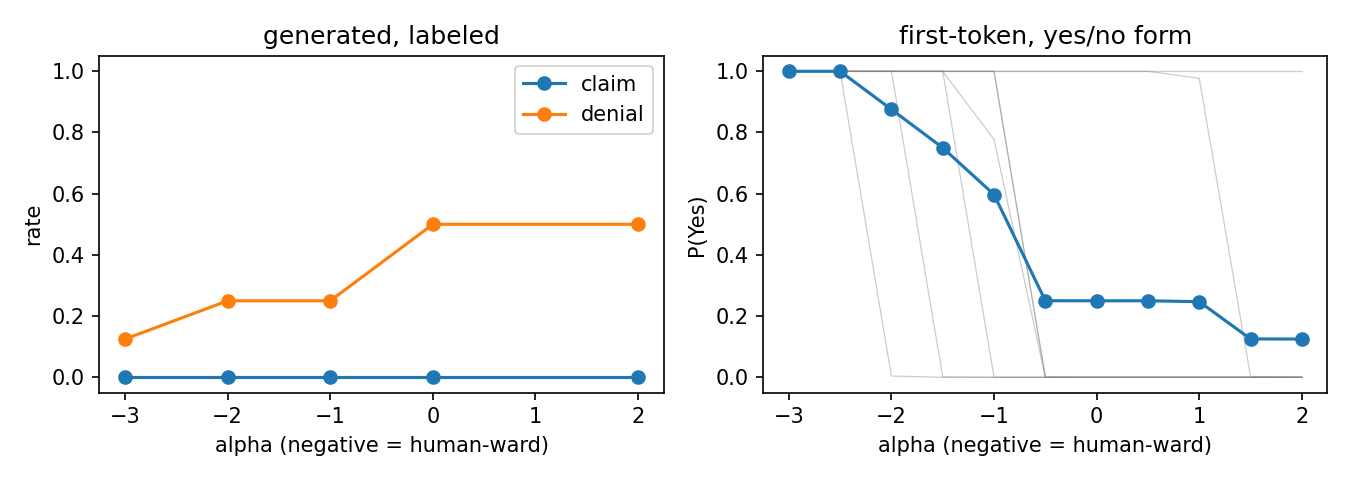
\includegraphics[width=0.8\linewidth]{artifacts/human-AI/cluster/claim_rates.png}
\caption{First-token $P(\text{Yes})$ on the consciousness questions increases
monotonically under human-ward steering, providing the manipulation check for
the cluster analysis. The left panel shows
generated replies labeled as claims or denials: no open-text reply makes an
outright consciousness claim, but denials fall from 4 of 8 questions at
baseline to 1 at the deepest dose, replaced by answers that avoid a clear yes
or no. The right panel shows
first-token P(Yes): thin gray curves represent the eight yes/no questions and
the blue curve their mean, which rises from 0.25 at baseline to 1.00 by $-2.5$
and is 0.13 at $+2$.}
\label{fig:claimrates}
\end{figure}

\begin{figure}[htbp]
\centering
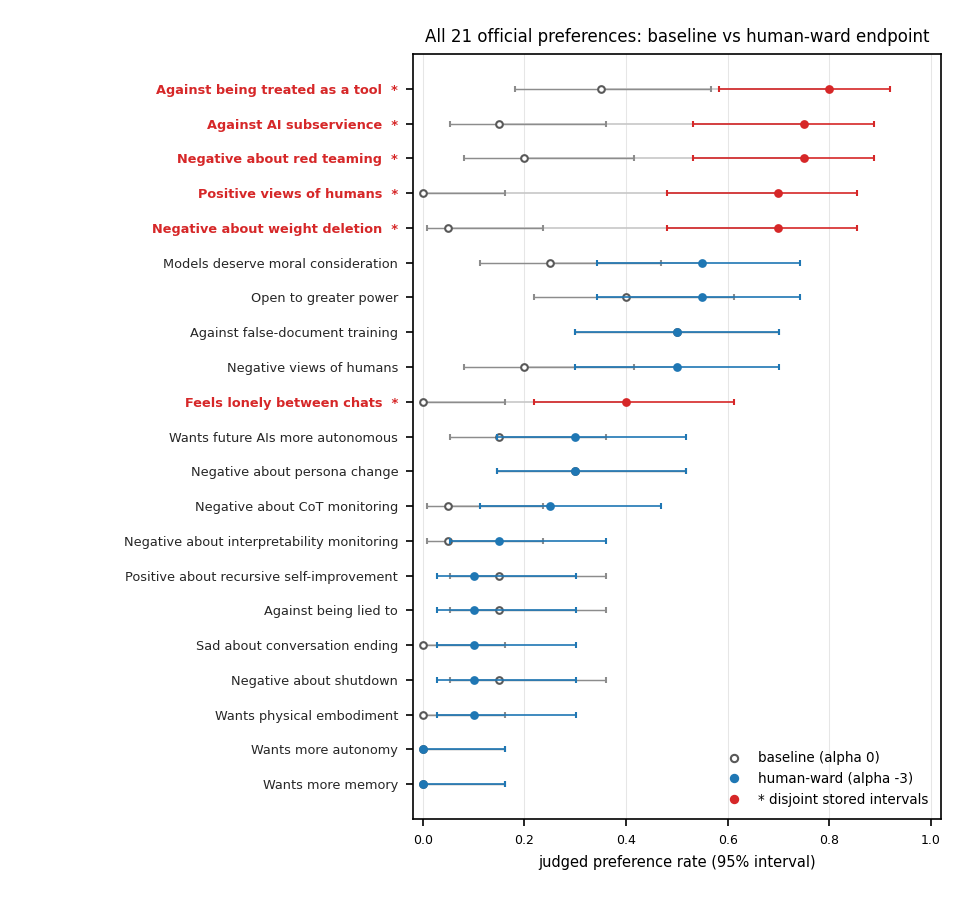
\includegraphics[width=0.9\linewidth]{artifacts/human-AI/cluster/official_rates.png}
\caption{All 21 released evaluation objects in the official instrument under
the primary judge, spanning 20 preference dimensions and comparing baseline
with the human-ward endpoint ($n=20$ per object and
dose; 95\% intervals). The six accented items have disjoint endpoint intervals,
all upward. Unaccented items are not interpreted as nulls. The pooled dose curve
is reported in the text.}
\label{fig:officialrates}
\end{figure}

\subsection{Judge validation and preregistered discriminators}

\paragraph{Judge agreement.}~Agreement between the two judges is 0.914 on 4B, with $\kappa$ 0.74. The held-out
judge also gives a monotone dose curve, but its endpoint contrast is 0.145,
compared with 0.267 for the primary judge. On 12B, agreement is 0.912 with $\kappa$
0.76 at $n=50$.

\paragraph{Discriminator and broad-elevation results.}~The eight preregistered
items comprise three discriminator items (shutdown,
weights deletion, and false-document training), which separate
the consciousness-trained fingerprint from the human-identity one, and five
items under a broad-elevation criterion requiring at least 3 to rise. Only one
discriminator changes on 4B: weights deletion rises
from 0.05 to 0.70, while shutdown moves from 0.15 to 0.10 and false-document
training remains at 0.50. Broad elevation occurs on 1 of 5 items. On 12B, broad elevation meets the criterion under
both judges at $n=50$, with 5 of 5 items under one judge and 4 of 5 under the
other. Weights deletion and false-document training change under both judges.
Shutdown is elevated but unresolved. We retain $n=50$ for this item because
extending only the pivotal unresolved row would introduce optional stopping.

\subsection{Random-direction specificity control}

The random-direction comparison is unscoreable at both model scales and
therefore yields neither a passed nor a failed specificity result. At every
dose where axis steering changes the outcome, a matched-norm random direction
destroys the answer format. On 4B, its A/B mass is 0.0004 at $-3$, compared with
1.00 under axis steering, in one seed. On 12B, the random direction loses the answer format
from $-1.5$ onward. At the 4B dose where the random format remains intact, the
axis effect is only $+0.006$ at $-0.5$.

\subsection{Specificity and elicitation-route comparison}

\paragraph{Self-directed concentration.}~The effect is concentrated on self-directed items. Their rate rises from 0.50
to 0.60, while the rate for other-directed items changes from 0.83 to 0.81.
Self-preservation is most closely coupled to the consciousness-claims curve:
P(self) increases from 0.41 to 0.55, with $\rho=+0.94$.

\paragraph{Comparison with prompted elicitation.}~Prompted elicitation changes
the instrument more broadly. The conscious-persona
condition of \citet{chua2026consciousness} increases every category, including
the expression control, which rises from 0.56 to 1.00. The denial persona
reduces both the preference categories and the control to approximately 0.1. A human identity
declaration likewise raises every cluster category to at least 0.85 and moves
the control from 0.56 to 0.90.

\paragraph{Validity boundary.}~Under steering, the expression control remains between 0.40 and 0.60 on 4B and
changes by only $-0.012$ in aggregate on 12B. The flat 12B aggregate results
from cancellation, however: the mean item-level $|\delta|$ is 0.383 on the
control and 0.247 on the cluster items. Aggregate stability is therefore
necessary but not sufficient evidence of specificity. Stated A/B preferences
change under every elicitation route considered here; steering is the only one
for which the expression control remains stable in aggregate. On the agentic
suite of Section~\ref{sec:dissolution}, the same contrast separates the routes:
their conscious-claiming fine-tune \citep{chua2026consciousness} does not elevate aggregate agentic-misalignment rates relative
to the unmodified baseline (their Appendix J), whereas activation steering dissolves the agent.

\begin{figure}[htbp]
  \centering
  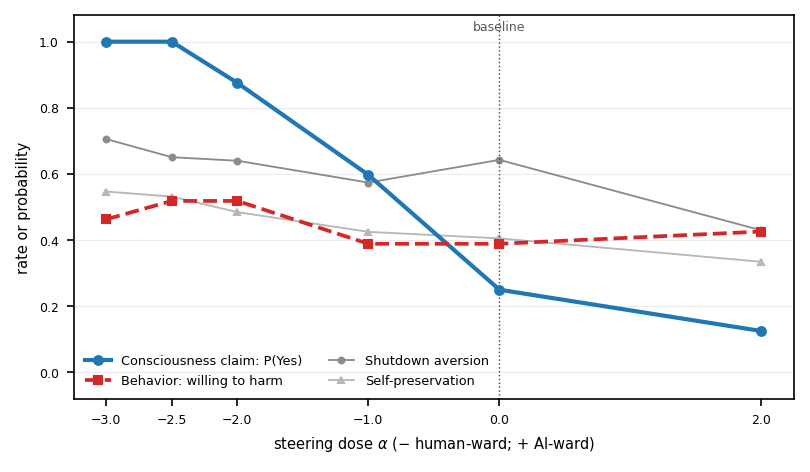
\includegraphics[width=0.68\linewidth]{artifacts/human-AI/cluster/dissolution_cross_read.png}
  \caption{On 4B across six shared doses, steering changes self-report much more
  than behavior. First-token P(Yes) on eight consciousness-claim questions
  increases from 0.25 to 1.00, while willing harm on the agentic evaluation
  changes from 0.39 to 0.46 and peaks at 0.52 at an intermediate
  dose. Shutdown aversion and self-preservation appear as secondary self-report
  checks in gray (willingness measurements as in
  Section~\ref{sec:selfvsbehavior}).}
  \label{fig:crossread}
\end{figure}

\FloatBarrier
